% Figure: Segment structure diagram
\begin{figure}[H]
\centering
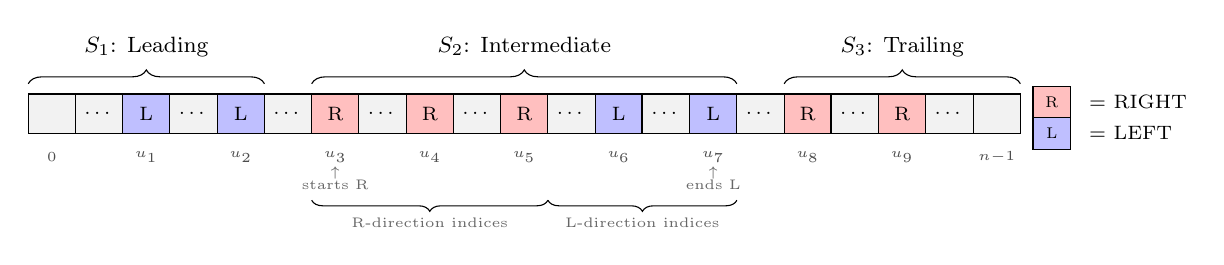
\begin{tikzpicture}[
    cell/.style={minimum width=0.6cm, minimum height=0.5cm, draw, font=\scriptsize},
    dotcell/.style={minimum width=0.5cm, minimum height=0.5cm, font=\scriptsize},
    indexcell/.style={minimum width=0.6cm, font=\tiny, text=black!70},
    right/.style={cell, fill=red!25},
    left/.style={cell, fill=blue!25},
    clean/.style={cell, fill=gray!10, font=\scriptsize},
    segbrace/.style={decorate, decoration={brace, amplitude=5pt}},
    segbracem/.style={decorate, decoration={brace, amplitude=4pt, mirror}},
    seglabel/.style={font=\footnotesize},
    condlabel/.style={font=\tiny, text=black!60},
    faded/.style={opacity=0.4}
]

% Array indices (shown below)
\def\yidx{-0.55}
\def\yarr{0}

% === ARRAY START ===
\node[clean] at (-0.9, \yarr) {};
\node[indexcell] at (-0.9, \yidx) {$0$};
\node[clean] at (-0.3, \yarr) {\dots};

% === LEADING SEGMENT (L's only, bounded by array start) ===
\node[left] (l0) at (0.3, \yarr) {L};
\node[indexcell] at (0.3, \yidx) {$u_1$};
\node[clean] at (0.9, \yarr) {\dots};
\node[left] (l1) at (1.5, \yarr) {L};
\node[indexcell] at (1.5, \yidx) {$u_2$};

% Inter-segment clean region
\node[clean] at (2.1, \yarr) {\dots};

% === MIDDLE SEGMENT (R's then L's) ===
\node[right] (r1) at (2.7, \yarr) {R};
\node[indexcell] at (2.7, \yidx) {$u_3$};
\node[clean] at (3.3, \yarr) {\dots};
\node[right] (r2) at (3.9, \yarr) {R};
\node[indexcell] at (3.9, \yidx) {$u_4$};
\node[clean] at (4.5, \yarr) {\dots};
\node[right] (r3) at (5.1, \yarr) {R};
\node[indexcell] at (5.1, \yidx) {$u_5$};
\node[clean] at (5.7, \yarr) {\dots};
\node[left] (l2) at (6.3, \yarr) {L};
\node[indexcell] at (6.3, \yidx) {$u_6$};
\node[clean] at (6.9, \yarr) {\dots};
\node[left] (l3) at (7.5, \yarr) {L};
\node[indexcell] at (7.5, \yidx) {$u_7$};

% Inter-segment clean region
\node[clean] at (8.1, \yarr) {\dots};

% === TRAILING SEGMENT (R's only, bounded by array end) ===
\node[right] (r4) at (8.7, \yarr) {R};
\node[indexcell] at (8.7, \yidx) {$u_8$};
\node[clean] at (9.3, \yarr) {\dots};
\node[right] (r5) at (9.9, \yarr) {R};
\node[indexcell] at (9.9, \yidx) {$u_9$};

% === ARRAY END ===
\node[clean] at (10.5, \yarr) {\dots};
\node[clean] at (11.1, \yarr) {};
\node[indexcell] at (11.1, \yidx) {$n{-}1$};

% === SEGMENT BRACES (top) ===
% Leading segment
\draw[segbrace] (-1.2, 0.38) -- (1.8, 0.38);
\node[seglabel] at (0.3, 0.85) {$S_1$: Leading};

% Middle segment
\draw[segbrace] (2.4, 0.38) -- (7.8, 0.38);
\node[seglabel] at (5.1, 0.85) {$S_2$: Intermediate};

% Trailing segment
\draw[segbrace] (8.4, 0.38) -- (11.4, 0.38);
\node[seglabel] at (9.9, 0.85) {$S_3$: Trailing};

% === SUB-BRACES for middle segment (bottom) ===
\draw[segbracem] (2.4, -1.1) -- (5.4, -1.1);
\node[condlabel, anchor=north] at (3.9, -1.2) {R-direction indices};
\draw[segbracem] (5.4, -1.1) -- (7.8, -1.1);
\node[condlabel, anchor=north] at (6.6, -1.2) {L-direction indices};

% === ANNOTATIONS for boundary conditions ===
% Condition markers (centered on cells)
\node[condlabel] at (2.7, -0.75) {$\uparrow$};
\node[condlabel] at (2.7, -0.9) {starts R};

\node[condlabel] at (7.5, -0.75) {$\uparrow$};
\node[condlabel] at (7.5, -0.9) {ends L};

% === LEGEND ===
\node[right, scale=0.8] at (11.8, 0.15) {R};
\node[font=\scriptsize, anchor=west] at (12.15, 0.15) {= RIGHT};
\node[left, scale=0.8] at (11.8, -0.25) {L};
\node[font=\scriptsize, anchor=west] at (12.15, -0.25) {= LEFT};

\end{tikzpicture}
\caption{A segment $(i,j)$ starts at either index $0$ or an R-direction updated index, and ends at either index $n{-}1$ or an L-direction updated index, with all R's preceding all L's within. In this example, the leading segment $S_1$ contains only L's (starting from index $0$), the intermediate segment $S_2$ contains R's followed by L's, and the trailing segment $S_3$ contains only R's (ending at index $n{-}1$). Leading and trailing segments may or may not be present depending on the directions of updated indices.}
\label{fig:segment-structure}
\end{figure}